\documentclass[12pt]{article}
\usepackage{color}
\usepackage{graphicx}
\usepackage[margin=1.0in]{geometry}
\newcommand{\hilight}[1]{\colorbox{yellow}{#1}}
\newcommand{\figref}[1]{Figure \ref{#1}}

\begin{document}
\begin{titlepage}
\title{\textbf{CPSC 504 Project\\\vspace{3 cm}\Huge{An investigation into an application to manage data transformations and updates}\vspace{2 cm}}}
\date{\vspace{2 cm} April 14, 2015}

\author{
 \makebox[1.0\linewidth]{Laura Cang}\\cang@cs.ubc.ca\\
  \and \makebox[1.0\linewidth]{Kailang Jiang}\\jiangkl@cs.ubc.ca\\
  \and \makebox[1.0\linewidth]{Jessica Wong}\\jhmwong@cs.ubc.ca\\ 
}
\maketitle
\thispagestyle{empty}
\end{titlepage}

\newpage
\section{Introduction}
\label{sec:introduction}
This project builds on the theoretical framework described in the M.Sc thesis of Arni Thrastarson \cite{arniThesis} and focuses on the first of the four scenarios detailed in the work. The first scenario investigates how changes made by a data application can be captured and propagated to a remote data source. The main workflow of this scenario involves a (possibly third party) application pulling the data from a remote data source to use locally. In order to facilitate updates to the data source, the application receives a schema mapping to identify the source table(s) of the data attributes along with a copy of the data it is requesting. The user using the application after retrieving the data may choose to add, remove, or edit the data. These changes are then logged to a transformation script which is later used to update the main copy of the data in the remote data store.

In this project, we focus on three different ways a user can use the application to fetch data. For the rest of this paper, we shall call each of the following a sub-scenario. 
\begin{enumerate}
	\item {When the user chooses to view all the columns in one table}
	\item {When the user chooses to view a subset of the columns in one table}
	\item {When the user chooses to view a subset of columns in multiple tables}
\end{enumerate}

\noindent Our primary contributions are:
\begin{enumerate}
	\item{Defining a data transformation language using logical programming concepts to capture changes made to a relational data model}
	\item{Proposing how the data source could react and handle schema changes}
	\item{Investigating view maintenance policies for the remote data source}
	\item{Detailing scenarios in which an application views a subset of columns from one or more tables in a remote data source}
	\item{Deciding on the division of responsibility between the database administrator and the application user in regards to data updates}
\end{enumerate}

\section{Motivation}
\label{sec:motivation}
We believe that the three sub-scenarios outlined are realistic. The first sub-scenario can be easily envisioned when thinking about a librarian trying to re-catalogue all the books in a library. The librarian would need to have all the information about a book in order to catalogue and double check the information.

As a motivating example for using a subset of one table, we consider a school administrator who is deciding to which student to award an academic merit prize.  The school administrator could go to the main database storing all student information (e.g., name, student number, GPA, guardian contact information, date of birth, allergy/medication information, family doctor contact, etc.) but only wishes to access student number and GPA columns to ensure that the prize is awarded fairly.

Lastly, users might need to view a subset of columns in multiple tables if they are a journalist intern who has been tasked with compiling a report for an online journal. The report could be on differences in critic ratings and user ratings for animated movies produced in the last five years which would require the intern to look at information from a movies and user information table.. 

\subsection{Sample data used in our project}
In our project, we decided to borrow the dataset used in CPSC 304, an introductory relational database course at UBC, to use as the test dataset in our application.  Specifically we use the ``MOVIESTAR'' table, which has three columns ``STARID'', ``NAME'', and ``GENDER''. After supplementing some additional data to the dataset, namely the columns ``MOVIE TITLE'', ``PRODUCTION STUDIO'', and ``CRITIC RATING'', we used this dataset. We then created a second table detailing user information using the column ``Movie Title'' as a foreign key to reference the ``MOVIE TITLE'' column in the Movie Information table, ``SOURCE WEBSITE OF USER INFORMATION'', ``USER RATING'', and ``NUMBER OF LIKES''.

\section{Solution}
The basic workflow of the scenario described in Section \ref{sec:introduction} remains the same. However, as the user obtains more flexibility over what columns can be chosen to view in his/her application,  the complexity of the data transformation increases due to the amount of information that must be tracked (see Section \ref{sec:transformation_language}). In this project, we have decided to support the following user changes: adding a column, removing a column, renaming a column, editing a table cell's value, removing a table cell's value, adding a row, and removing a row. Any changes that cause a violation in schema definitions (e.g., removing a row's primary key) will be resolved on the server side by the database administrator. This design decision was due to not wanting to restrict the types of users that would be able to use an application to explore and update data. As we have to assume that there could be users unfamiliar with schema/storage restrictions, we decided to ensure that schema violations are resolved by someone with the technical understanding of what error has occurred. 

\subsection{Types of Changes Supported}
\label{sec:types_of_changes}
We have decided to focus on two of the eight changes mentioned in Wrangler \cite{kandel2011wrangler}: map and reshape. Map changes deal with ``[transforming] one input data row to zero, one, or multiple output rows'' \cite{kandel2011wrangler}. This essentially means that the row changes that are supported in our application (e.g., add row, delete row, edit value(s) in row(s)) all fall within this class of changes. Reshape changes deal with schema changes. Any change to the columns (e.g., add/remove/rename columns) will fall into this category. The scope of this project does not deal with changing the data type of a column.

\subsection{Transformation Language}
\label{sec:transformation_language}
During the design of the transformation language, we realized that it did not make sense to start with the simplest of our three sub-scenarios as the transformation language did not scale well with increasing complexity. Therefore, we are basing our decisions around the most complicated of our three sub-scenarios: the situation where an application has pulled a subset of columns from more than one table.  To ensure that the transformations worked for the simpler sub-scenarios, every step was aligned with all consequences in mind.

When designing the data transformation language, we decided to emulate some of the logical programming concepts from Prolog (none too biased by our instructor's well-known preference for Datalog).  We primarily borrowed from the syntactical style and the easy-to-understand format. The addition of a timestamp was in preparation for a possible future extension of the project where multiple concurrent users would make updates to the data source. Table \ref{table:transformations_summary} has a summary of how the structure of each data transformation will look like for each function.

\begin{table}[!ht]
\centering
\begin{tabular}{ | c | l | }
 \hline
    User Action & Data Transformation Syntax \\ \hline \hline
    Add Row & addRow(tableName(columnName1:valuesUserPutIn1,\\ & columnName2:valuesUserPutIn2, \\ & ..., \\ & columnNameN:valuesUserPutInN),  timestamp)\\ & \\ \hline
    Remove Row & removeRow(tableName(primaryKey1:primaryKeyValue1,\\ & primaryKey2:primaryKeyValue2, \\ & ..., \\ & primaryKeyN:primaryKeyValueN),  timestamp)\\ & \\ \hline
    Add Column & addCol(tableName, nameOfNewCol, timestamp)\\ & \\ \hline
    Remove Column & removeCol(tableName, nameOfColToRemove, timestamp)\\ & \\ \hline
    Rename Column & renameCol(tableName, oldNameofCol, newNameOfCol, \\ & timestamp)\\ & \\ \hline
    Edit Value & editValue(tableName(originalPrimaryKey, ..., originalPrimaryKeyN,\\ & columnNameOfEditedValue1:editedValue1, \\ & columnNameOfEditedValue2:editedValue2, \\ & ..., columnNameOfEditedValueN:editedValueN),  timestamp)\\ 
    \hline
\end{tabular}
\caption{The data transformations logged to the transformation script as the user makes changes to the data.}
\label{table:transformations_summary}
\end{table}

\noindent The rest of this paper will use the following tables:
\begin{itemize}
\item {Movie Information(Movie Title: String, Primary Key; Movie Debut Year: Int; Production Studio: String, not null; Total Gross: double; Critic Rating: String)}
\item{User Information(Movie Title: String, Foreign Key; Website that user information was obtained from: String, Primary Key; User Rating: String; Number of Likes: double)}
\end{itemize}

Once an application has pulled data from a remote database, the resulting set of columns shown in the application will be referred to as a view. For the journalist intern example mentioned in Section \ref{sec:motivation}, the columns being viewed are ``MOVIE TITLE'', and ``CRITIC RATING'', both of which come from the Movie Information table, ``USER RATING'', ``NUMBER OF LIKES'', and ``SOURCE WEBSITE OF USER INFORMATION'' columns, which come from the User Information table. The Movie Information table has ``MOVIE TITLE'' as the primary key while the User Information table has ``MOVIE TITLE'' as its foreign key and ``SOURCE WEBSITE OF USER INFORMATION'' as its primary key. Table \ref{table:add_row_table_example} shows what the displayed view after the user has pulled from the remote database. Note that schema mappings are also pulled to the application along with the data from the remote database. The schema mappings will be used to help determine what tables each of the respective columns in the view belong to.

\begin{table}[!ht]
\centering
\begin{tabular}{ | c | c | c | c | c | }
 \hline
    Movie Title & Critic  & User & Number & Website that user\\
    & Rating & Rating & of Likes & information was \\
    &&&& obtained from\\ \hline \hline
    Despicable Me 2 & 5/5 & 5/5 & 220 000 & IMDB\\ \hline
    Up & 5/5 & 5/5 & 225 000 & Facebook\\ \hline
    Kung Fu Panda 2 & 4/5 & 5/5 & 500 000 & Rotten Tomatoes\\ \hline
    Mars Needs Moms & 3/5 & 3/5 & 103 000 & Rotten Tomatoes\\
    \hline
\end{tabular}
\caption{An example user-application display prior to the user making any changes to the data.}
\label{table:add_row_table_example}
\end{table}

A constraint on the view is that the primary key(s) of each table must be displayed.  This is a necessary detail as the primary key is needed to be able to uniquely identify the value being changed by the user (see Section \ref{sec:edit_value} for more details). Also, when a user decides to add a new row to the table (see Section \ref{sec:add_row} for more details), there needs to be values for the primary key(s) in order for a row to be added successfully. Allowing the user to choose which rows he/she wants does not guarantee that the primary key is chosen and this may result in a seemingly inexplicable loss of certain application functions. Therefore, when pulling information from each table, the application is required to pull all primary and foreign keys of the table. While we recognize that this will cause a lot of activity on the network and possibly take up more local memory, we could not think of a better solution. Due to this design decision, the example shown in Table \ref{table:add_row_table_example} does not include any details about whether the columns shown are the primary keys of their respective tables as we expect that the primary keys are already shown. There has been some discussion regarding how to make it easier for the user to determine primary key columns as opposed to other columns but we did not feel that non-technical users could understand the difference intuitively. For users that can understand why the idea of different columns belonging to different tables, it would certainly make it easier for them to perform actions such as add or remove a row (see Sections \ref{sec:add_row} and \ref{sec:remove_row}) but for the very non-technical users, it would only make it more distracting and confusing. Also, as we are possibly working with third party applications, we can only restrict what information gets pulled, we cannot expect anything in terms of how the information is visualized to the users.

\subsubsection{Adding a row}
\label{sec:add_row}
When the user uses his/her application to add a row in the view, it is unclear whether or not the user desires to include an additional row in all tables that have columns in the view. One of the design factors we have decided on is to include a new row in the tables that have a value filled in at the column. 

In Table \ref{table:add_row_table_example2}, the user has just added in a new row and populated the ``MOVIE TITLE'' and ``CRITIC RATING'' columns with a value. If the user decides to not populate the row any further and push his/her changes, the remote database would have the Movie Information table add a new row with Megamind as the ``MOVIE TITLE'' value and 3/5 as the ``CRITIC RATING'' value. However, as the Movie Information table has other schema restrictions, namely that the ``PRODUCTION STUDIO'' column must be populated, there will be an error generated when the user chooses to push to the remote database. We have decided to let the database administrator deal with issues like these at the remote database end. The alternative solution is to impose another restriction upon the application such that it will have to also pull columns that have schema specifications like ``unique'' or ``not null''. However, we felt that it would be too confusing for the end-user to have such columns included. With primary/foreign keys, the information captured in those columns gives the requisite context and meaning to rest of the information in that row. Columns that have schema specifications may not have such context and meaning and thus would be confusing to impose at the application end.

In Table \ref{table:add_row_table_example3}, the user has added more information about the movie ``Megamind''. As columns from the Movie Information table and the User Information table have been filled with values, there will be a new row added to the Movie Information and User Information table. Any issues with adding to the Movie Information table (e.g., missing a value for a column denoted not null in the database) will have to be resolved by the local database administrator. Changes that are definitely going to be rejected (e.g., adding in a row without a value for the primary key(s) will be rejected by the data source without needing input from the database administrator).

\begin{table}[!ht]
\centering
\begin{tabular}{ | c | c | c | c | c | }
 \hline
    Movie Title & Critic  & User & Number & Website that user\\
    & Rating & Rating & of Likes & information was \\
    &&&& obtained from\\ \hline \hline
    Despicable Me 2 & 5/5 & 5/5 & 220 000 & IMDB\\ \hline
    Up & 5/5 & 5/5 & 225 000 & Facebook\\ \hline
    Kung Fu Panda 2 & 4/5 & 5/5 & 500 000 & Rotten Tomatoes\\ \hline
    Mars Needs Moms & 3/5 & 3/5 & 103 000 & Rotten Tomatoes\\ \hline
    Megamind & 3/5 &  &  & \\
    \hline
\end{tabular}
\caption{The user is trying to add a new row to the table where only columns from the Movie Information table is filled.}
\label{table:add_row_table_example2}
\end{table}

\begin{table}[!ht]
\centering
\begin{tabular}{ | c | c | c | c | c | }
 \hline
    Movie Title & Critic  & User & Number & Website that user\\
    & Rating & Rating & of Likes & information was \\
    &&&& obtained from\\ \hline \hline
    Despicable Me 2 & 5/5 & 5/5 & 220 000 & IMDB\\ \hline
    Up & 5/5 & 5/5 & 225 000 & Facebook\\ \hline
    Kung Fu Panda 2 & 4/5 & 5/5 & 500 000 & Rotten Tomatoes\\ \hline
    Mars Needs Moms & 3/5 & 3/5 & 103 000 & Rotten Tomatoes\\ \hline
    Megamind & 3/5 & & 200 000 & IMDB \\
    \hline
\end{tabular}
\caption{The user is trying to fill in a new row that she has added. Columns from the Movie Information and User Information table have values added to them.}
\label{table:add_row_table_example3}
\end{table}

When the user adds a row, the change that is logged to the transformation script has the following structure: \\ \\
addRow(tableName(columnName1:valuesUserPutIn1, \\
 \indent columnName2:valuesUserPutIn2, \\
 \indent ..., \\
 \indent columnNameN:valuesUserPutInN), timestamp).

\subsubsection{Removing a row}
\label{sec:remove_row}
There are two methods for a user to delete a row in the data store. The first method involves selecting the ''Remove Row'' button while the second method is to delete all values from cells associated with that row in the table. Imposing only cell-at-a-time deletion when manipulating from the table helps avoid incidents where users accidentally delete whole rows when they just want to delete a single cell. We thought that this reflects how a user would normally use the system \textemdash if a user really wanted to delete a row, the whole row would be deleted anyways. As we felt that this accurately reflected a normal usage situation, we did not consider this as a constraint that imposed extra annoyance upon the user.

When the user removes a row by the ``Remove Row'' button, the change that is logged to the transformation script has the following structure: \\ \\
removeRow(tableName(primaryKey1:primaryKeyValue1, \\ 
\indent primaryKey2:primaryKeyValue2,\\
\indent ..., \\
\indent primaryKeyN:primaryKeyValueN), \\
\indent timestamp). \\ \\
We are use the primary key to identify which specific row to delete. The database system will handle delete propagation (i.e., deleting the rows that other tables have which use values referencing the ones in the deleted row).  

Removing values of all cells related to that row may also effectively delete the row.  Further value-editing details are described in Section \ref{sec:edit_value}.

\subsubsection{Adding a column}
\label{sec:add_col}
When adding a column, we considered two main possibilities: having a column added to all tables that have projections in the current view or adding to only one table.  Originally we chose to have the column added to all tables that have representation in the current view but quickly realized that it would lead to a lot of update problems including potentially increasing the number of otherwise null-valued rows. There would also be the problem of using extra memory. In the end, we decided to have the column added to the table with the most columns in the current view. If tables have an equal number of columns in the view, final destination for the column can be chosen in one of three ways:
\begin{itemize}
\item {Arbitrarily/at random}
\item {Based on the name of the table (e.g., add the column to the table with the name that is listed first when table names are sorted alphanumerically)}
\item {Based on the statistics of table usage that the database stores (e.g., the column could be added to the table that is queried more often). However, this would involve some back and forth dialog between the database and the remote application which may not be a good idea for performance or database security measures}
\end{itemize}

We decided to choose the second method to resolve any possible conflicts between table choice when adding columns. The add column change is logged as follows: \\ \\
addCol(tableName, nameOfNewCol, timestamp). 

\subsubsection{Removing a column}
\label{sec:remove_col}
While discussing this function, there was some concern about whether or not users should be allowed to remove a column and if they were, whether they should be allowed to remove primary key columns. In the end, we decided to only allow the removal of non-primary key columns for database security reasons. It could be argued that the user should be able to do whatever he/she wishes upon the data as that is the point of enabling users from all backgrounds to use and update data but upon weighing the pros and cons of this issue, it was decided that it was too easy for the user to cause major damage to the data source if primary key removal was allowed.  This would severely limit the availability and use of the data when scaled to allow for concurrent users.  Thus we decided on a requiring that users who wish to remove a primary key column would require the aide of the database administrator. The ''Remove Column'' change would be logged into the transformation script as follows: \\ \\
removeCol(tableName, nameOfColToRemove, timestamp).

\subsubsection{Renaming a column}
\label{sec:rename_col}
Although the situation where a user would rename a column is uncommon, we decided to enable support for this use case regardless. The transformation script syntax for this change is: \\ \\ renameCol(tableName, oldNameofCol, newNameOfCol, timestamp).

\subsubsection{Editing a value}
\label{sec:edit_value}
When editing a value, a user can make one of two types of changes, defined as follows:
\begin{itemize}
\item 1-1 \textemdash change from one value to another
\item 1-0 \textemdash value is deleted
\end{itemize}

As with the add row functionality (see Section \ref{sec:add_row}), if a user ends up violating schema constraints when editing a value, the database administrator will have to handle the changes. Some of the possible schema violations include changing a unique value to a non-unique one when the column specifies that it needs to have unique values or deleting a value from a column that has forbidden null values. The ''Edit Value'' change would be logged into the transformation script as follows: \\ \\ 

\noindent editValue(tableName(originalPrimaryKey1,.., originalPrimaryKeyN, \\
\indent columnNameOfEditedValue1: editedValue1, \\
\indent columnNameOfEditedValue2:editedValue2, \\
\indent ..., \\
\indent columnNameOfEditedValueN:editedValueN). \\ \\

The originalPrimaryKey1 to originalPrimaryKeyN variables hold the values of the primary keys for the row prior to any changes. The initial primary key values are needed to identify which row is to be changed; if one of the primary key values have been edited, we would not be able to correctly identify the rows to be changed without the initial primary key values.

\subsection{View Maintenance}
View maintenance is also something that factored into our considerations throughout the project. There were long discussions about whether or not we should allow the user to choose when updates would be pushed to the remote database or if the application should choose. In the end, we decided on a mixed-initiative approach where the user would push if certain types or a certain number of changes have occurred while also allowing the user to choose when to push changes. The primary concern was that schema changes were important enough to push right away (see Section \ref{sec:add_row}, \ref{sec:remove_row}, \ref{sec:add_col}, and \ref{sec:remove_col}) especially since we acknowledged that as the wait period grew, the potential effects of bad information grew accordingly. If this project is later extended to include multiple concurrent users, the longer schema changes are withheld, the greater the potential is for affecting a large number of users. Value changes are considered less important; for value changes that conflict from user to user, we elected to refer to the timestamp for resolution decision. The application can push to the remote data source after a threshold number of changes. We have left the definition of the automatic push threshold as a future work.

\subsection{Proof of Concept}
After designing the transformation language, we decided to implement the scenario from \cite{arniThesis} in order to show that our transformation language and design decisions could work to update a data source. A critical feature that we added was to allow for the user to choose which changes to sync to the remote data source. We created an interface using Netbeans that enabled users to load data from data source, make changes (while selecting whether to sync those changes), and push selected changes to remote data source.

\figref{fig:load} shows the original MOVIESTAR table data we extracted and loaded from the data source. We are only showing three columns: the first is a unique id of a movie star (i.e. the primary key of the table), the second is the name of the movie star, and the third is the gender of the actor. Currently, we only load the specific data and columns, but this can be easily extended to letting users choose which columns and rows to fetch. Every time ``Pull'' is clicked, we discard all the un-pushed changes and load the data from the remote data source.  Keeping the remote data source distinct from the application view means that a ''Pull'' without a ''Push'' is effectively a local ''Undo''.

\begin{figure} [!ht]
  \centering
  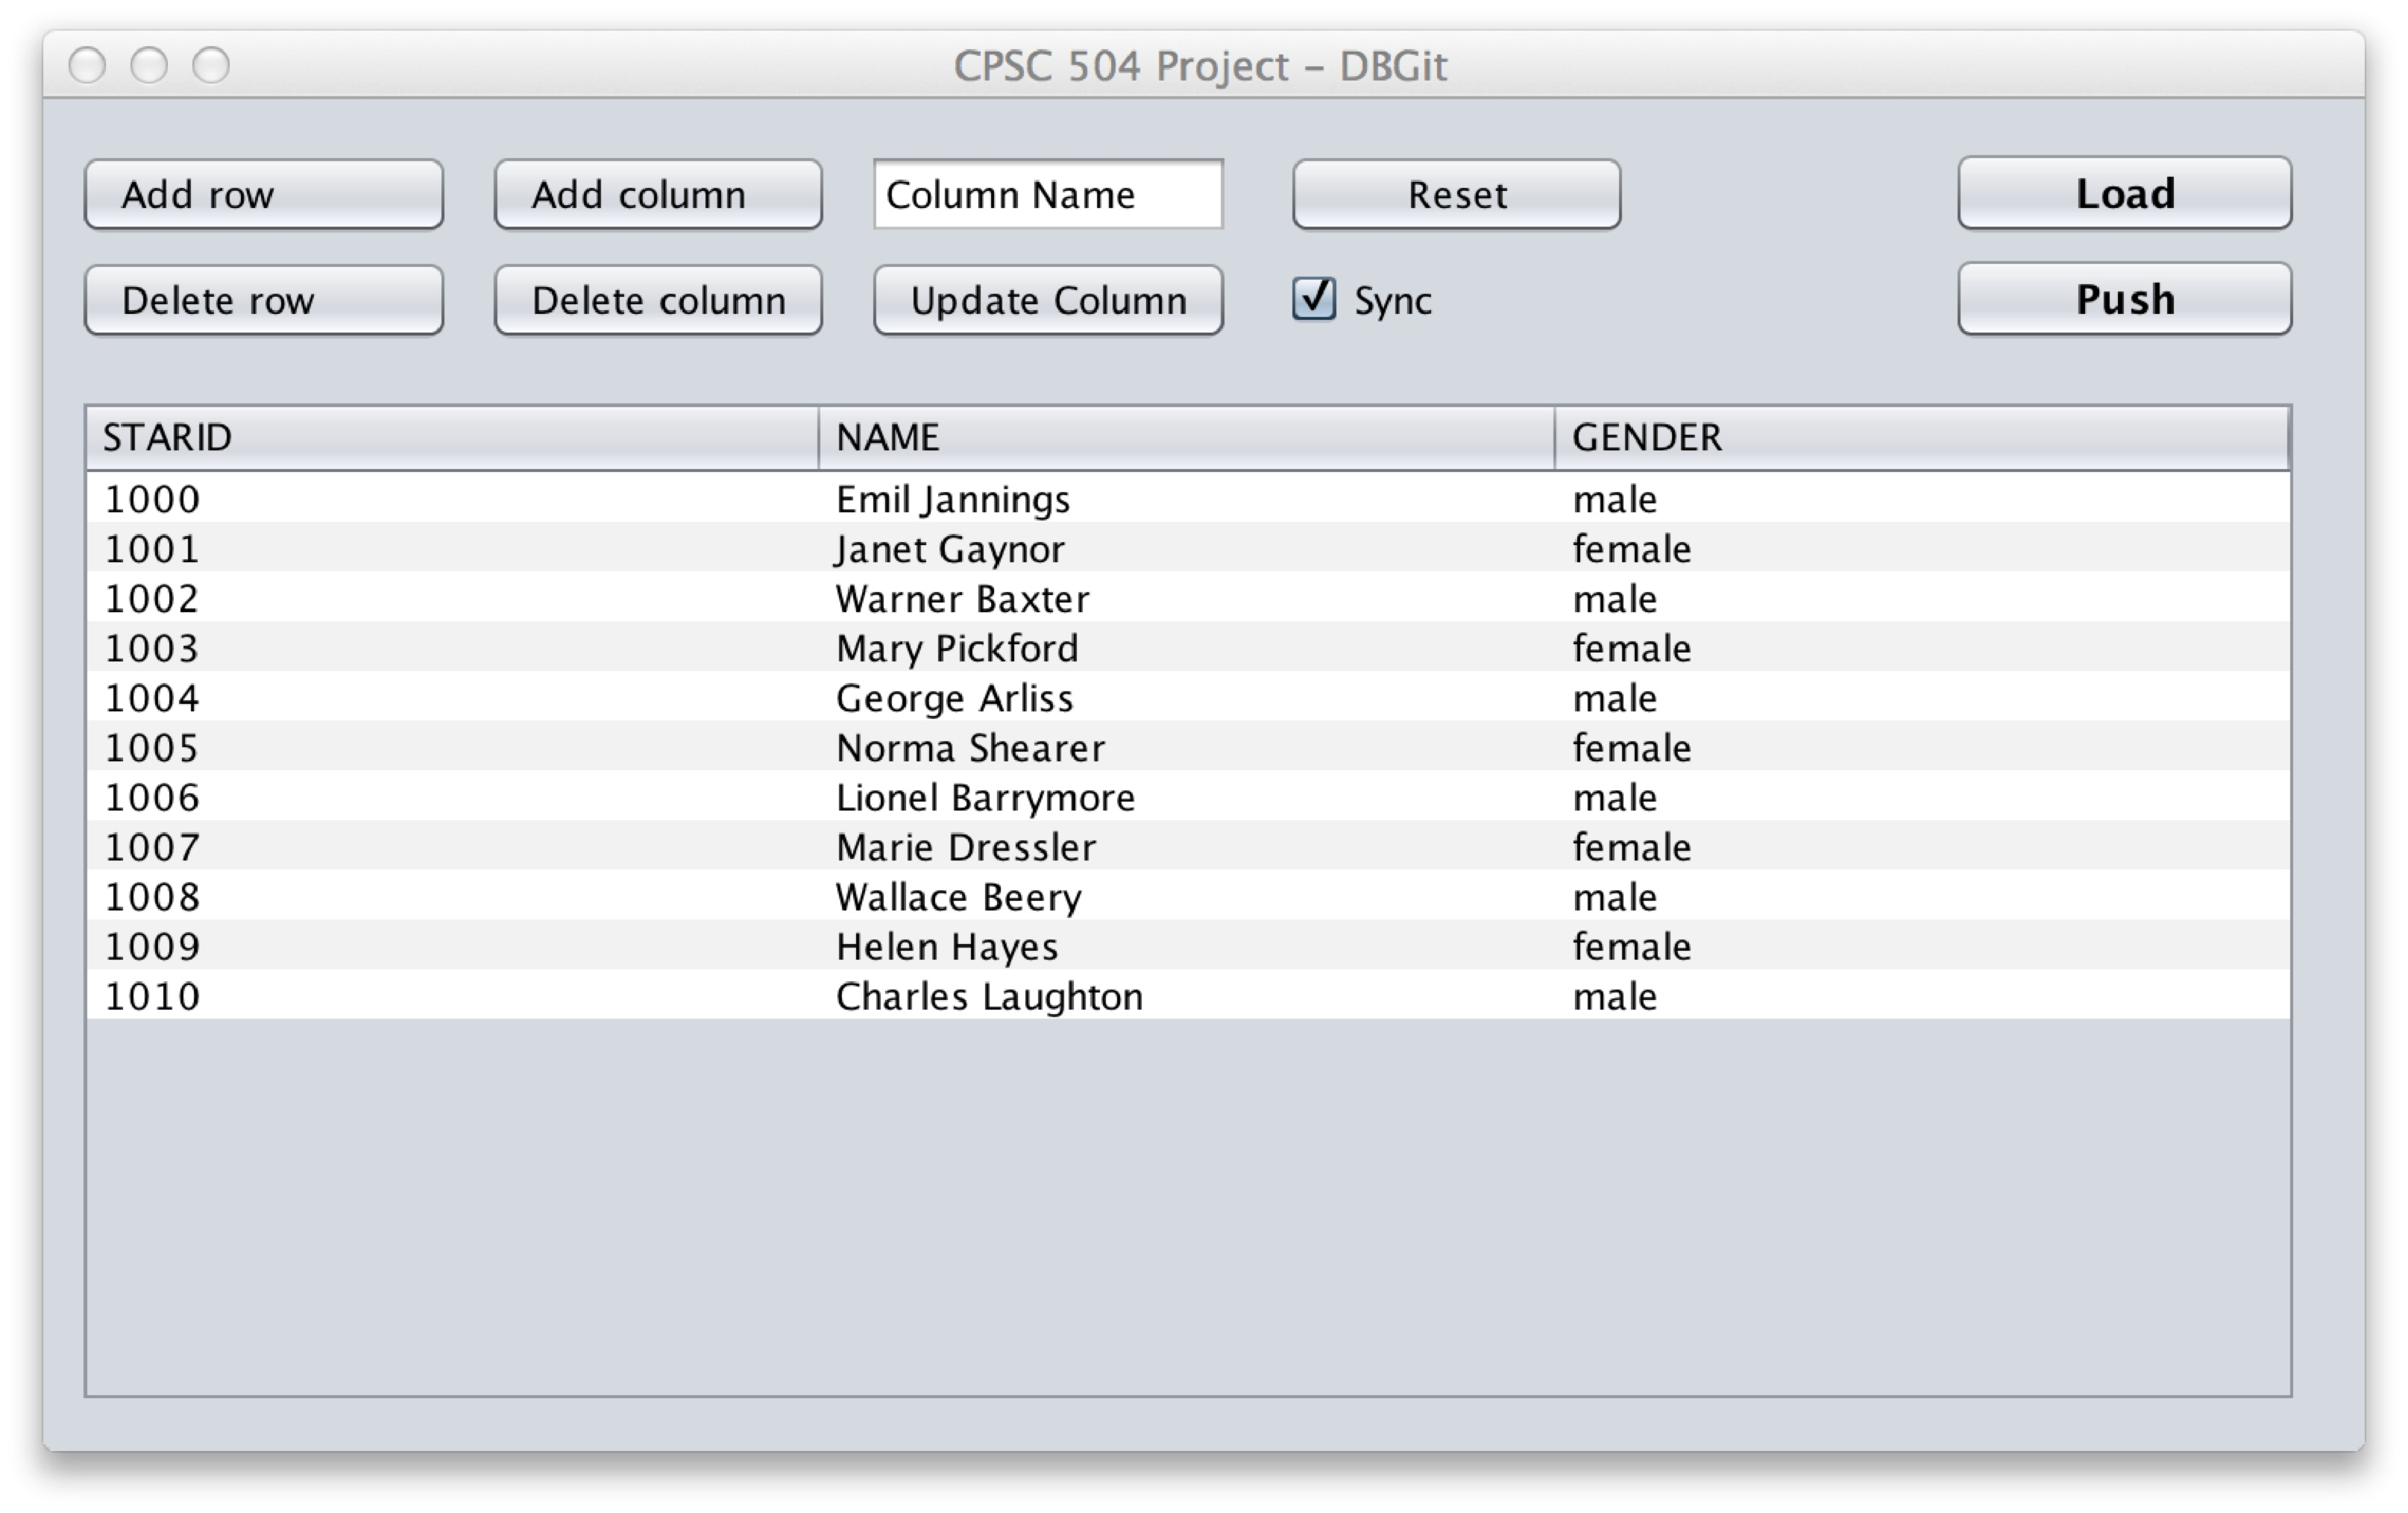
\includegraphics[width=0.9\columnwidth]{load}
  \caption{Original data loaded from remote data source}
  \label{fig:load}
\end{figure}

Now, we can try to make some changes. We will track all ``Map'' changes (i.e., adding/deleting a row, and editing the value) while ``Reshape'' changes (i.e.,  creating/delete/renaming a column) are only logged to the transformation script if the user wishes for the changes to be synced to the remote data source. \figref{fig:unsync} shows a few changes (add column ``height'' and ``weight'', and rename the first column to be ``ID'') we made to the original data that we chose to not sync and keep locally. \figref{fig:sync} shows some changes (add column ``age'', add a row, and update some cells) that we chose to log and sync. \\

\begin{figure}
  \centering
  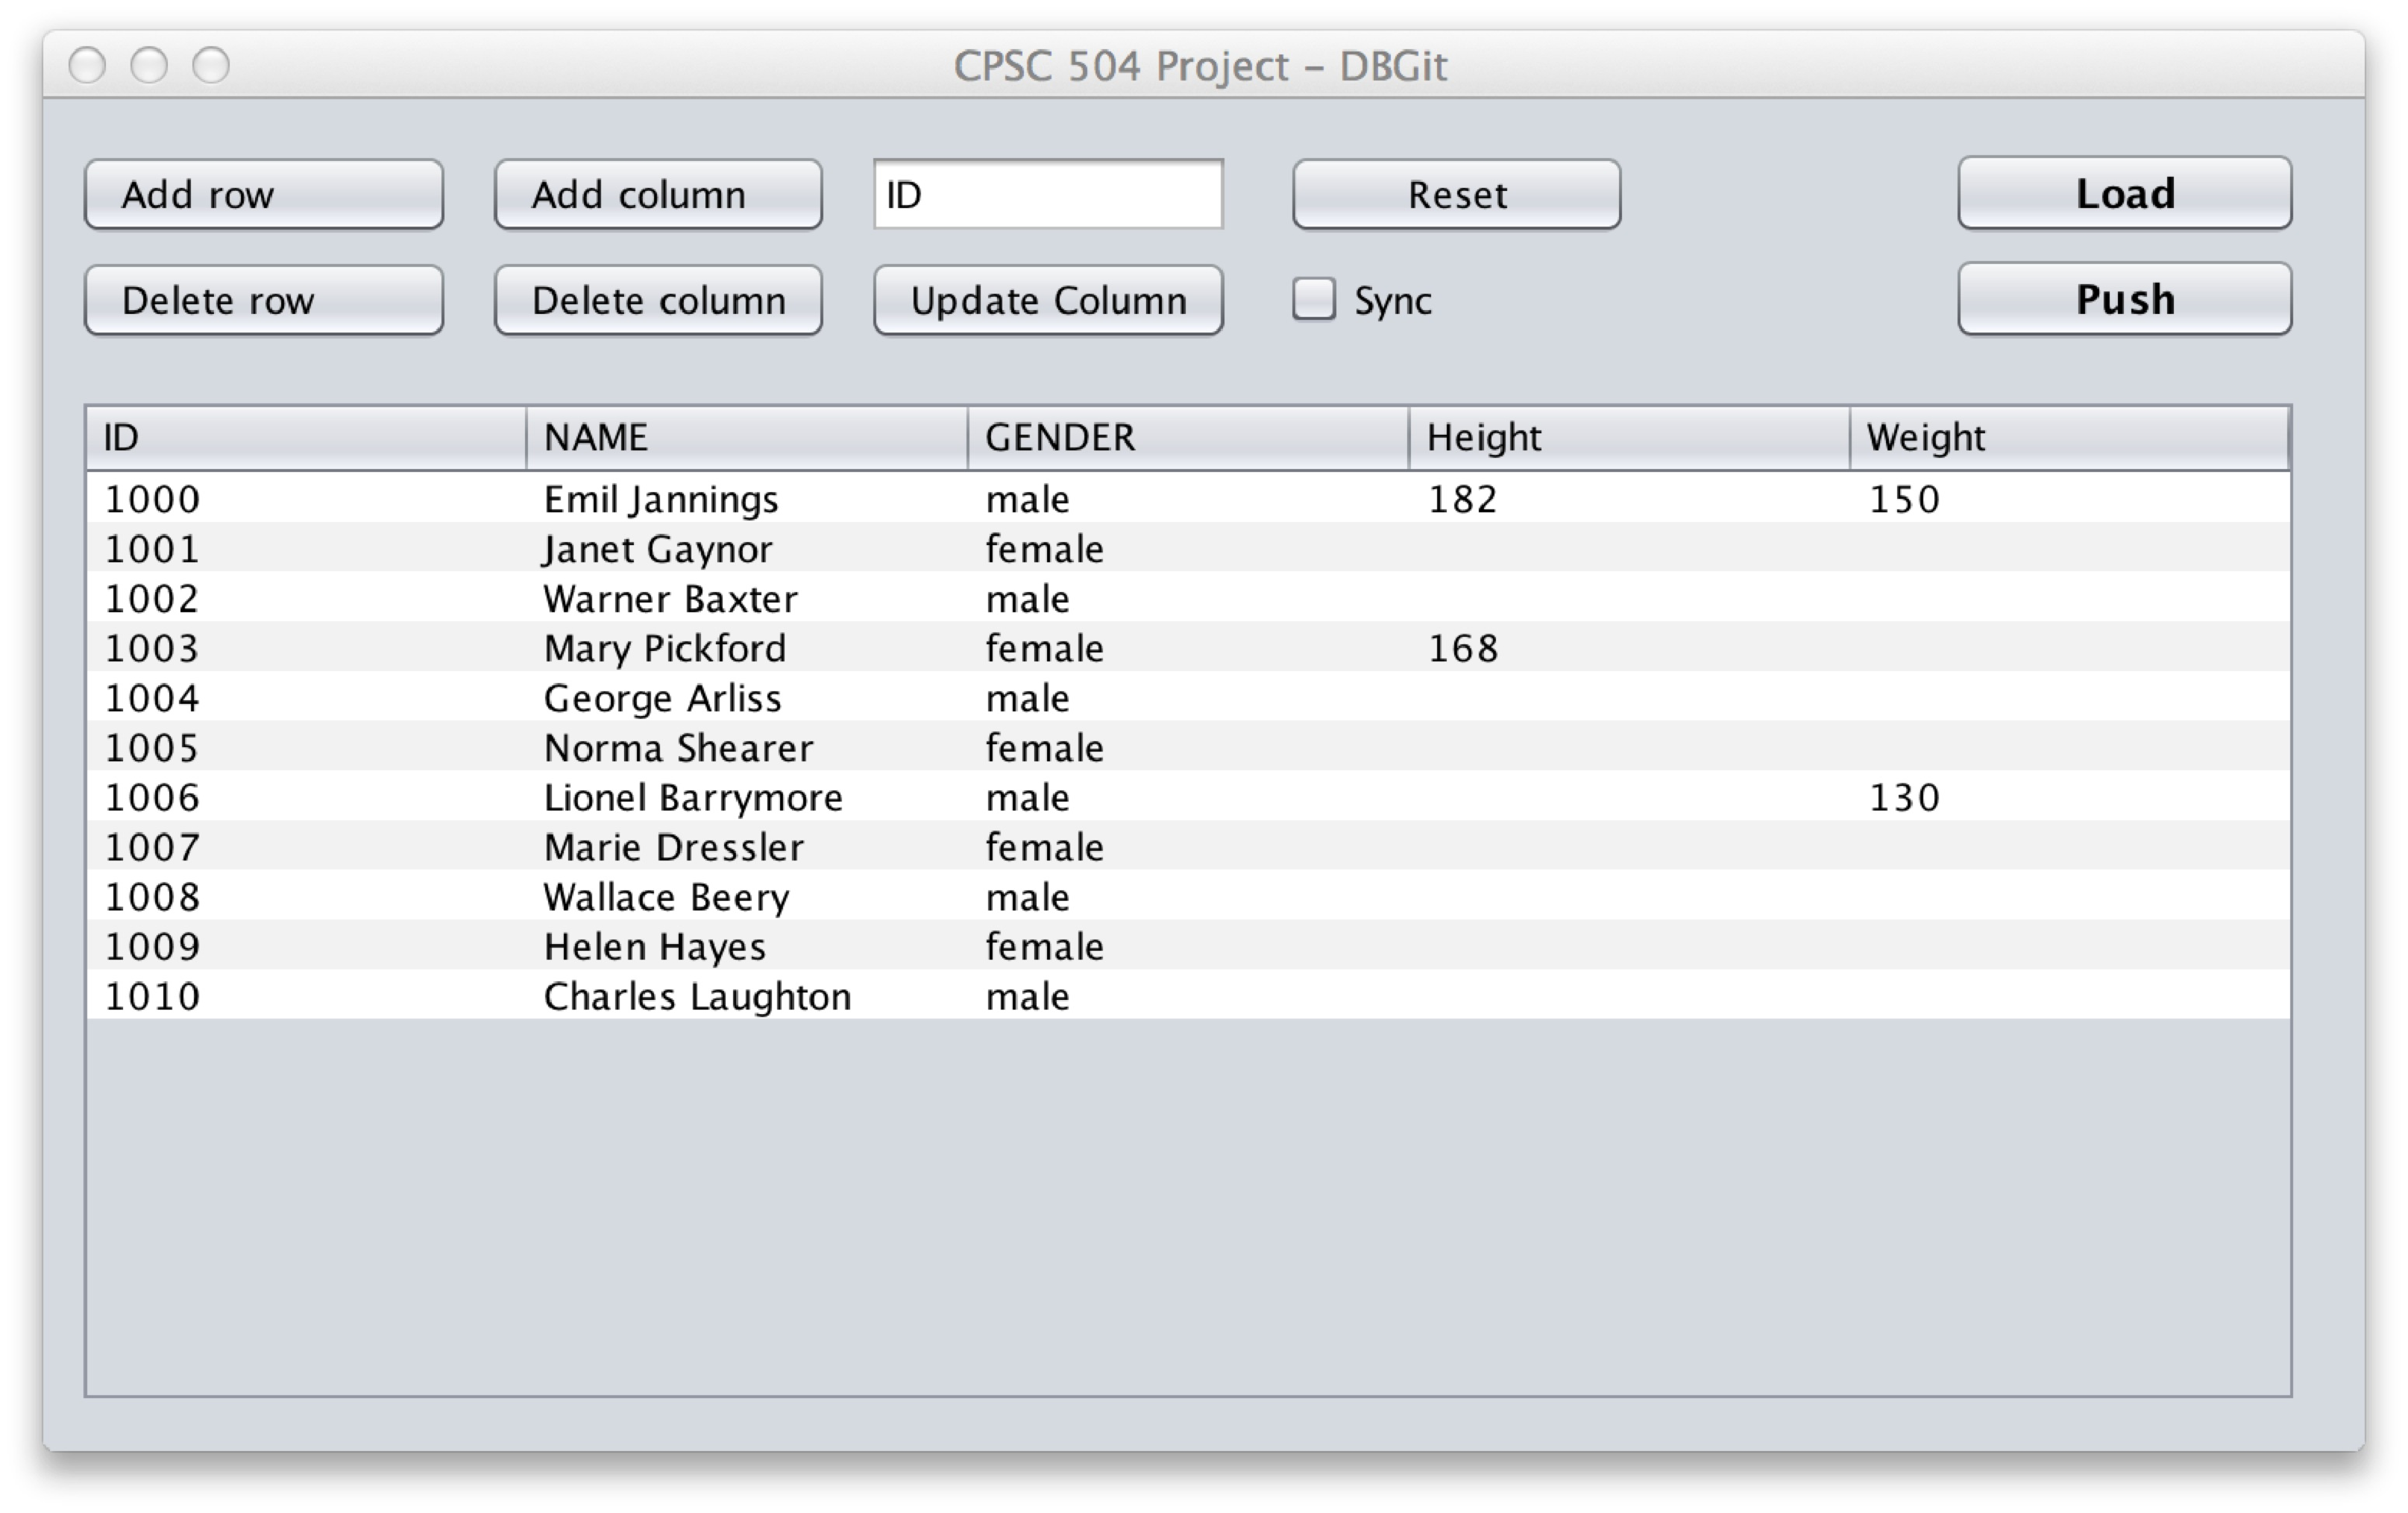
\includegraphics[width=0.9\columnwidth]{unsync}
  \caption{Changes that users choose not to sync}
  \label{fig:unsync}
\end{figure}

\begin{figure} [!ht]
  \centering
  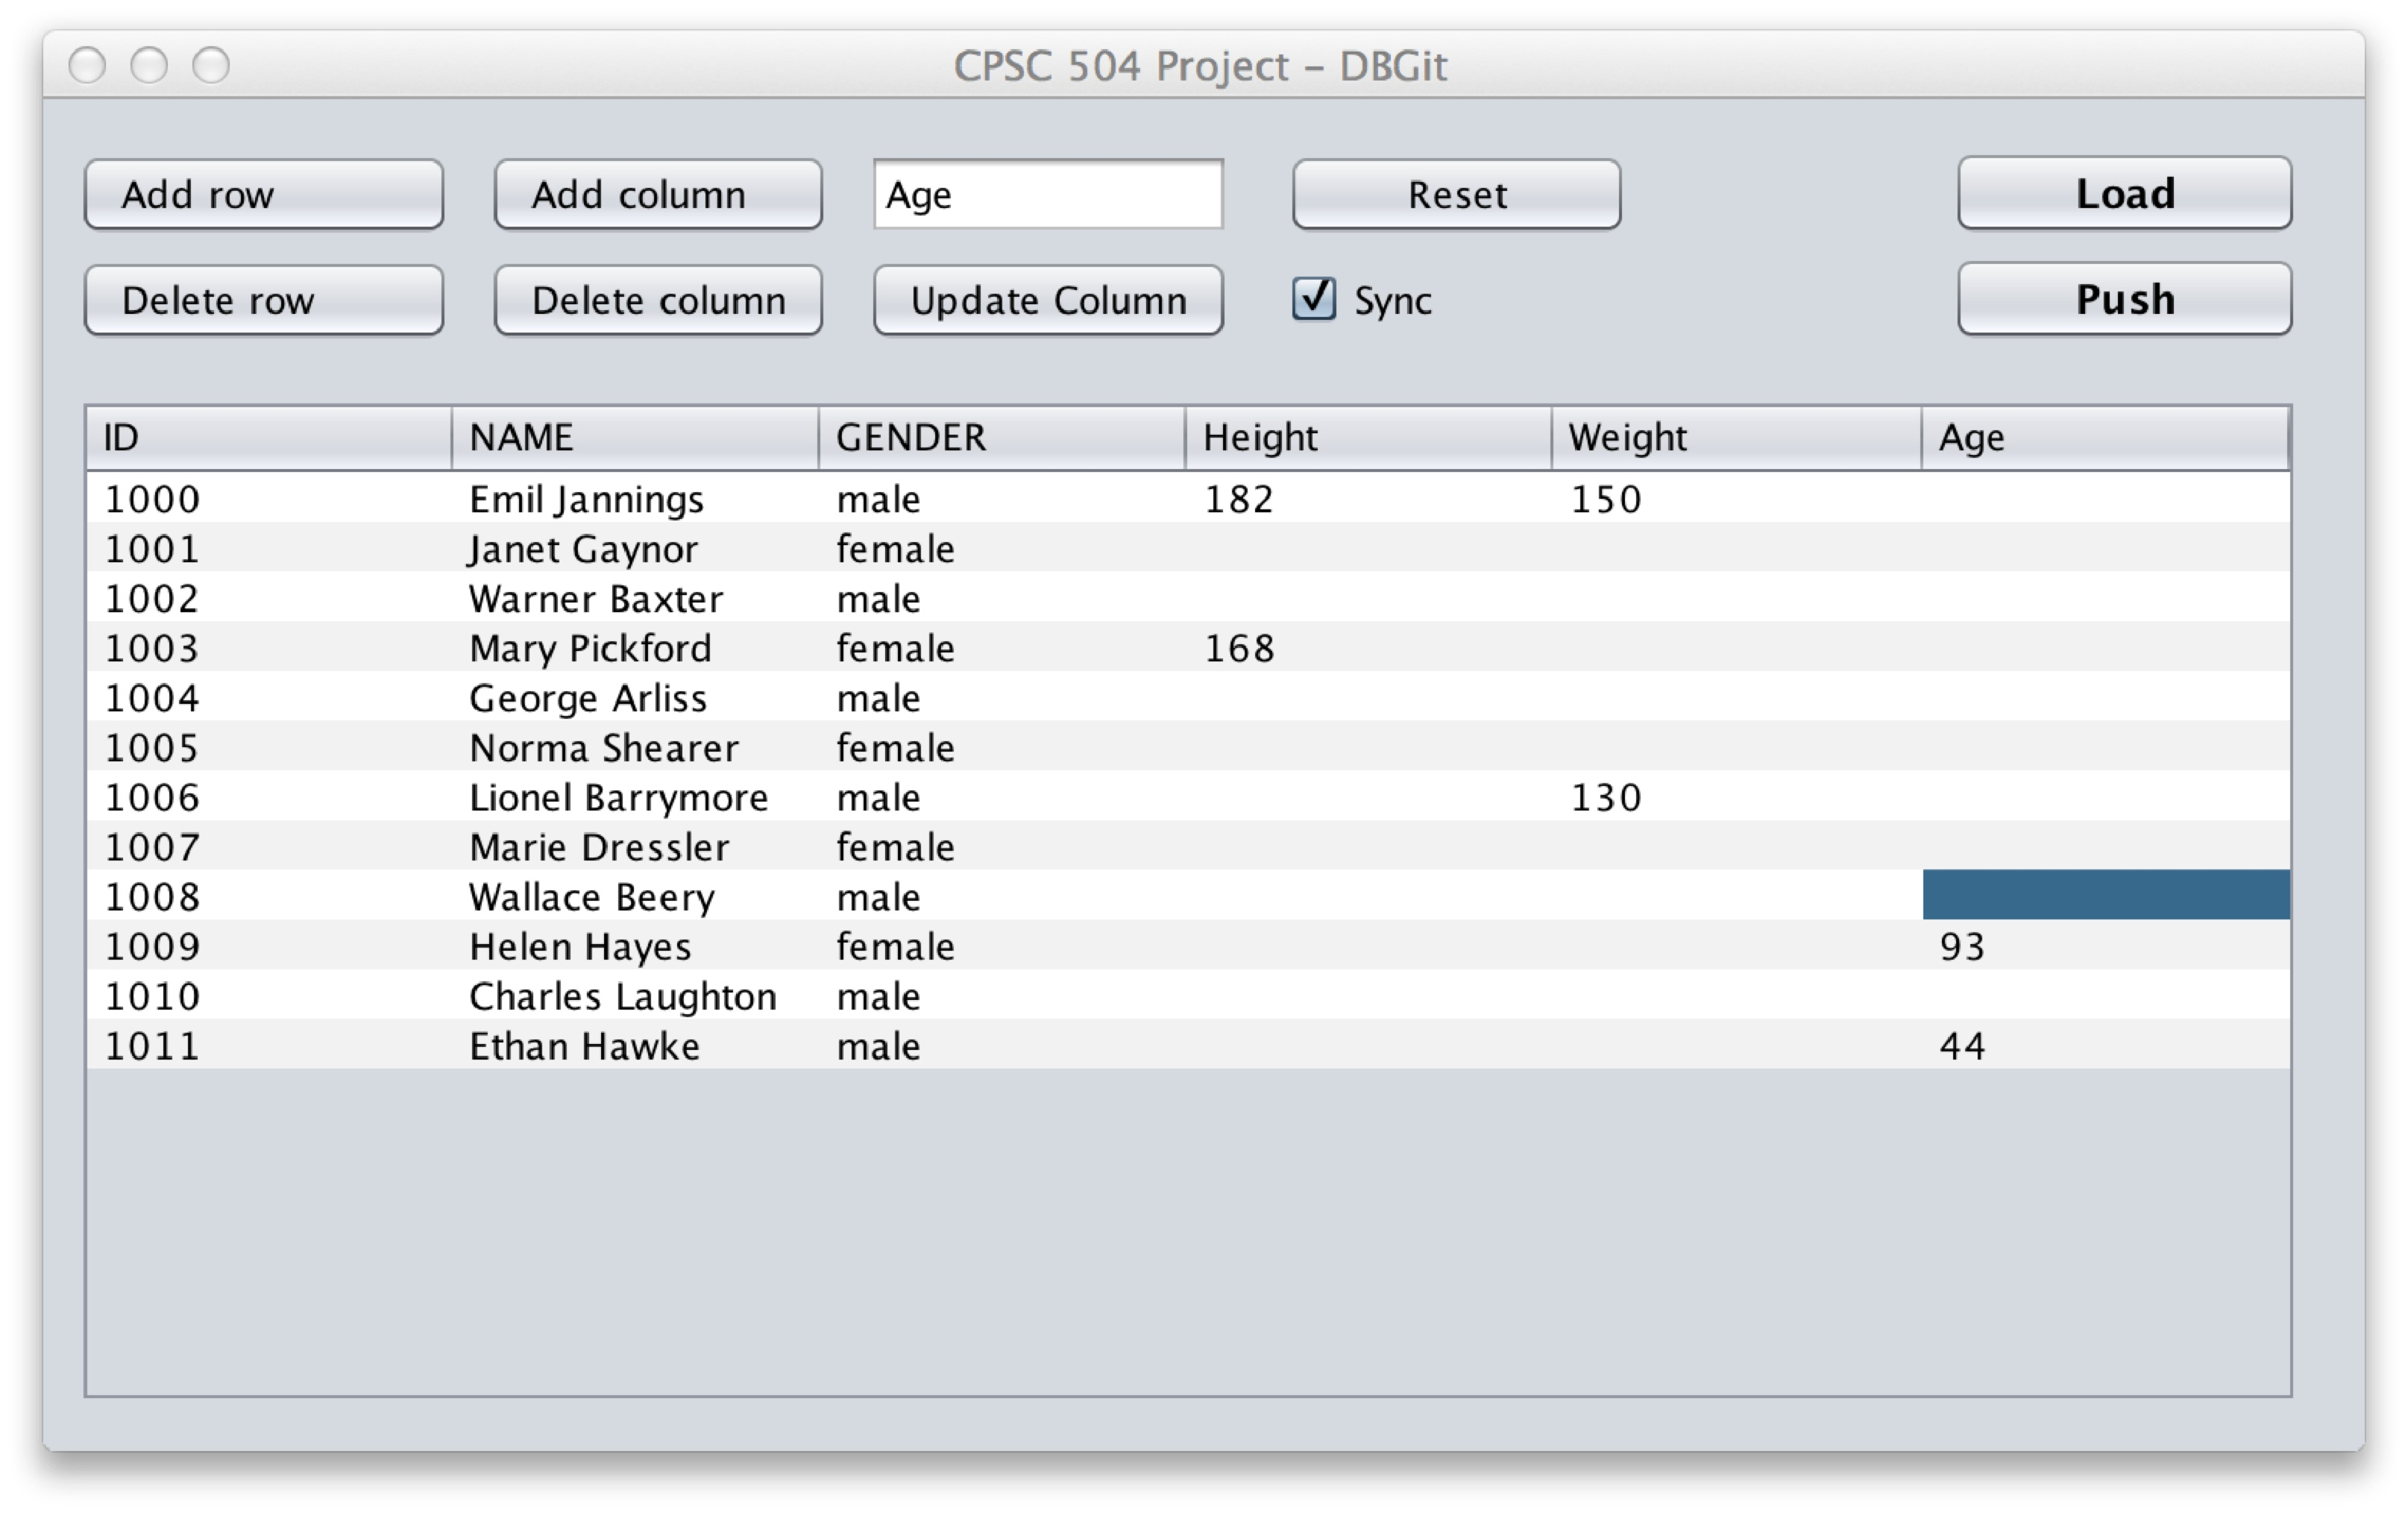
\includegraphics[width=0.9\columnwidth]{sync}
  \caption{Changes that will be logged and synced}
  \label{fig:sync}
\end{figure}
\newpage
Synced changes will not apply to the remote data source immediately. Instead, we generate a transformation script, and log every synced change to it using our transformation language. For example, operations in \figref{fig:sync} will be logged in our script and once the user selects the ``Push'' button, we will translate and and apply the transformation script to the remote data source. If we then click on ``Load'', the tool will load data in from the data source again (see \figref{fig:push}). We can see that the data loaded in from the data source is slightly different from the data we saw before reloading.  This is because only part of the changes made to our local data will be synced to the remote data source. If we load again, some changes we made to the local data copy will disappear.
%\newpage
\begin{figure} [!ht]
  \centering
  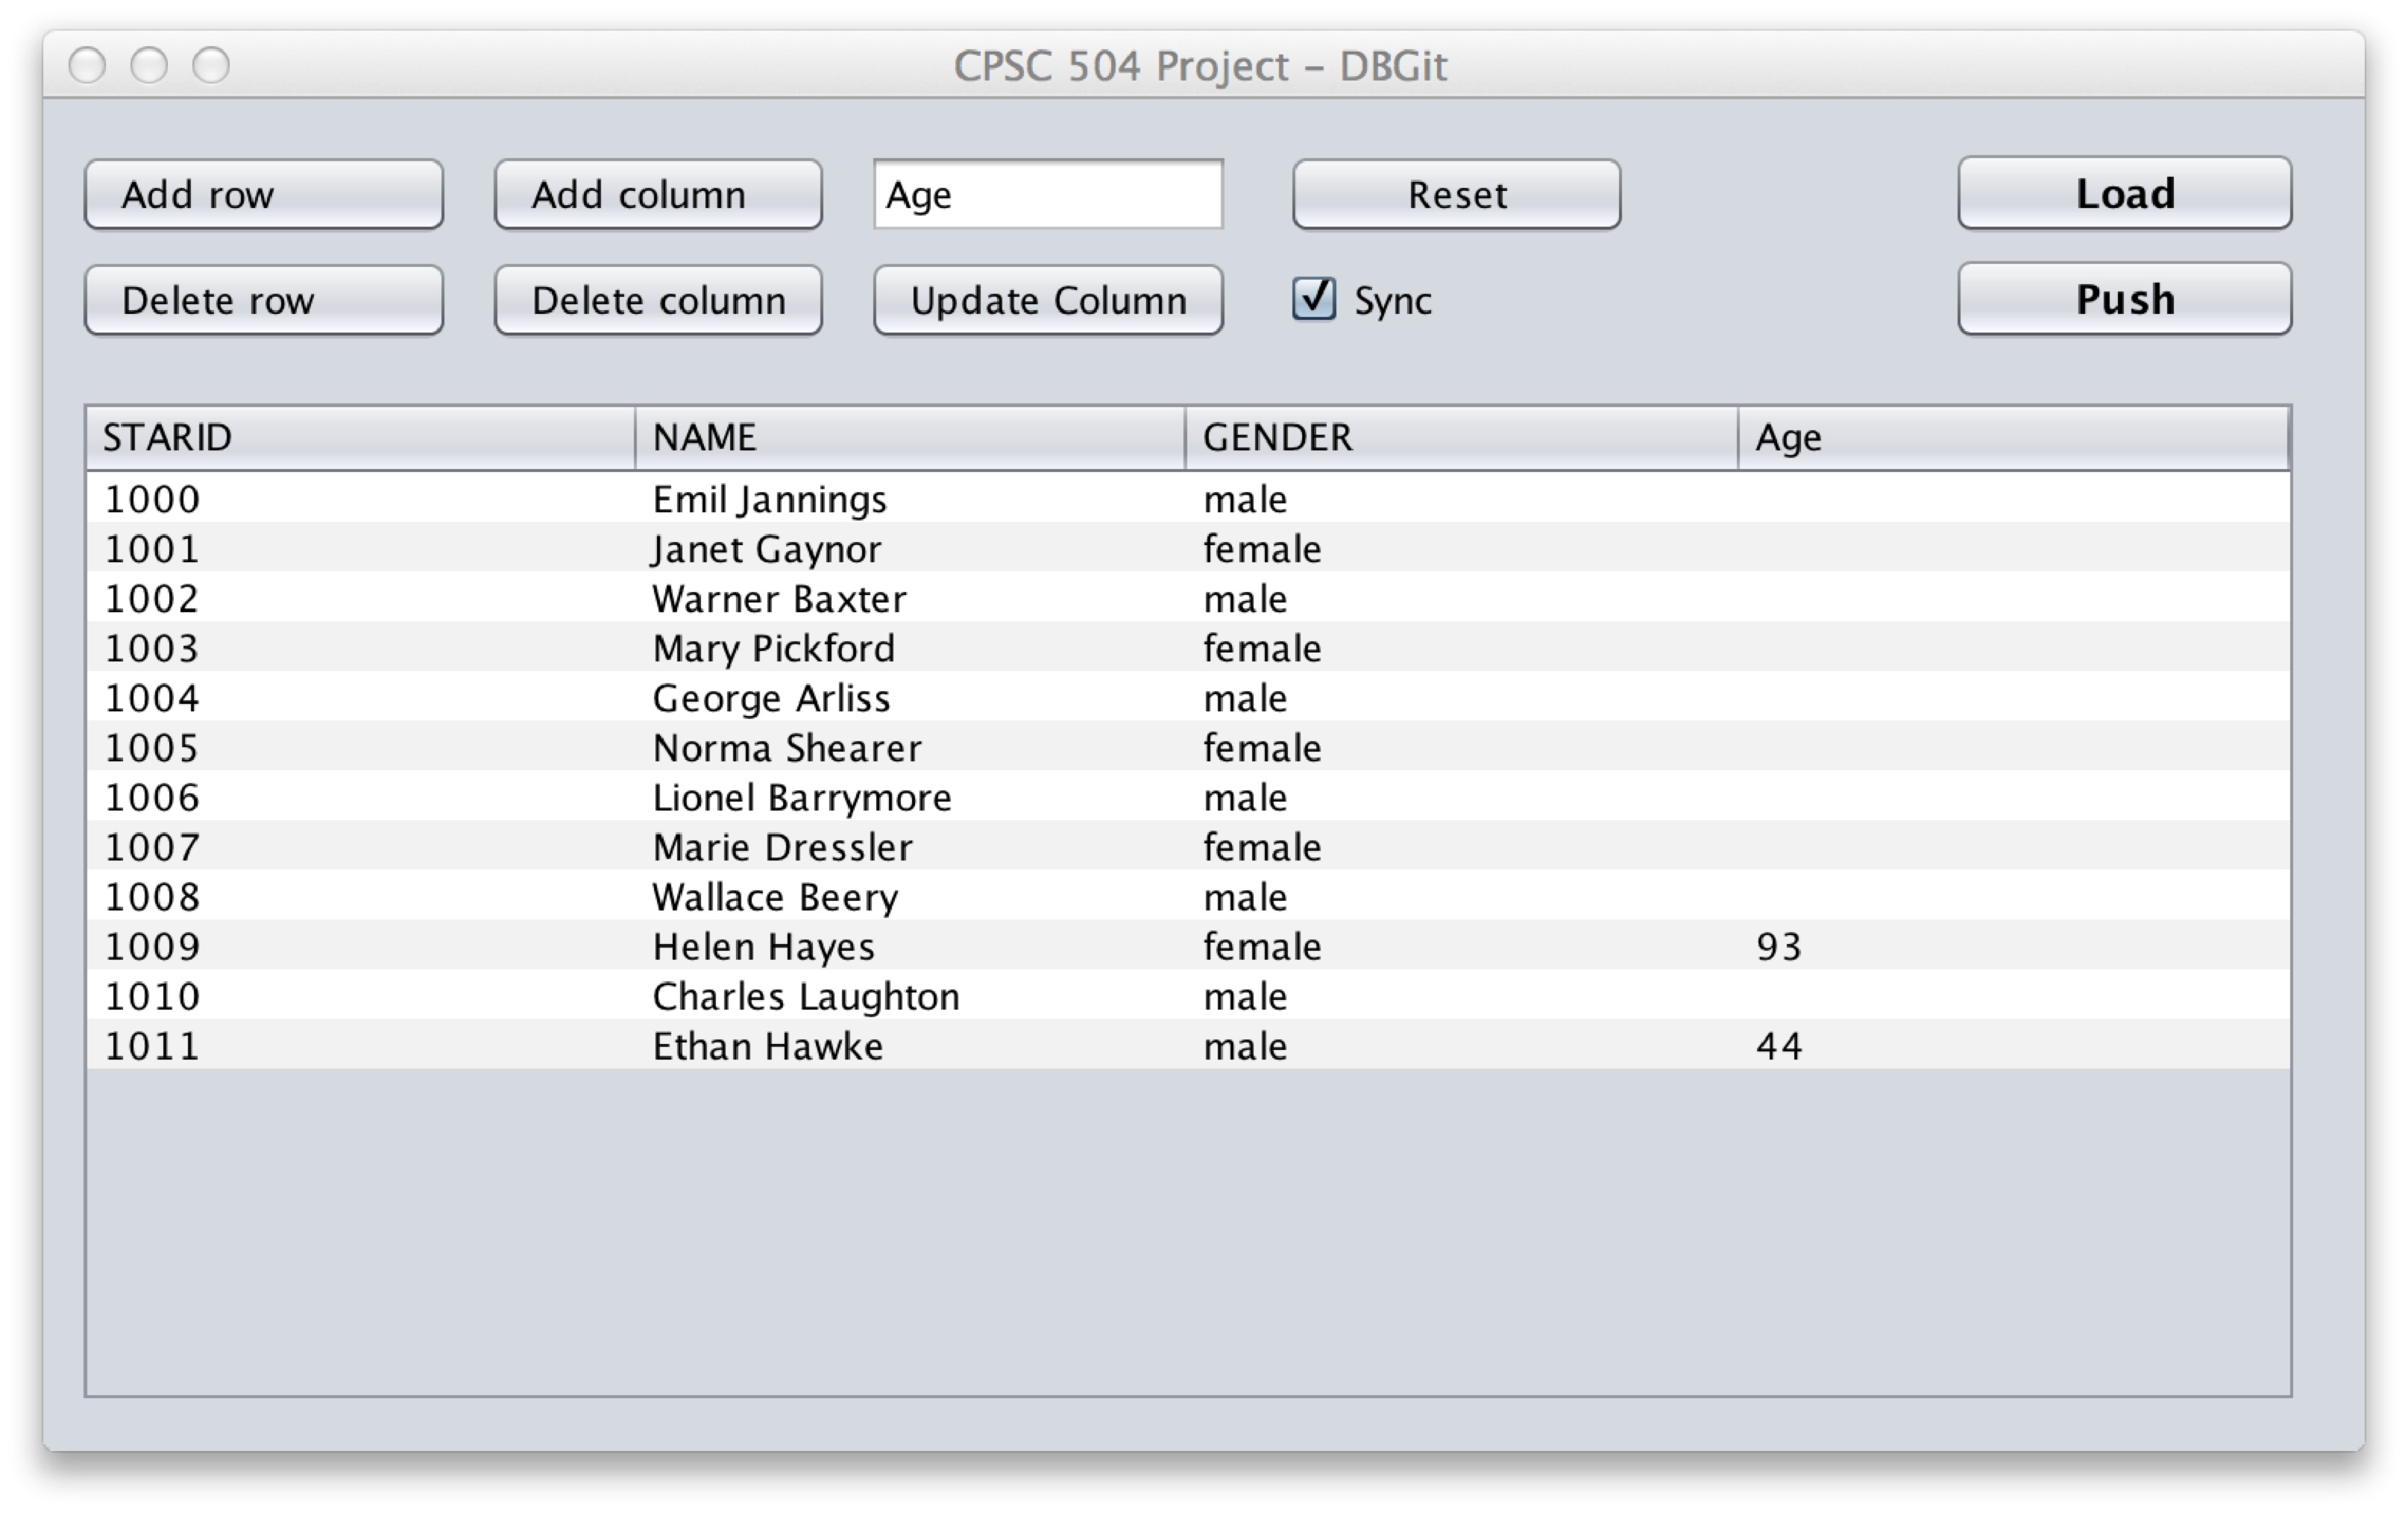
\includegraphics[width=0.9\columnwidth]{push}
  \caption{Modified data re-load from remote data source after push}
  \label{fig:push}
\end{figure}
%\clearpage



And also, the execution result of our transformation script and our translation of these scripts are proved to correct by comparing these results to the data set before we ``Push'' and re-``Load''.

%\newpage
\section{Related Work}
\subsection{Transformation Languages}
While there has been a large body of work done on various data transformation tools \cite{kandel2011wrangler, raman2001potter, kandel2012profiler}, these tools often focus on visualizing the data transformation rather than the transformation language used to represent the data changes behind the scenes. In fact, most of the work in the data transformation language domain seems to be classified into one of two categories. Either the work focuses on trying to help uses visualize the data transformations that have occurred \cite{kandel2011wrangler, raman2001potter, kandel2012profiler} or it focuses on modifying existing transformation languages to help with the data transformation process \cite{ilprints409, lakshmanan2001schemasql}. Due to the lack of literature about the specifics of data transformation languages, we decided to cast our net further and examine data transformation language frameworks. There was a minimal amount of literature on using logical programming concepts to create a data transformation language \cite{bry2002towards}. The idea was that people find declarative languages like logical programming languages easier to understand as it focuses on the relationships between the data models rather than the method of how to locate a certain piece of information to work with \cite{bry2002towards, tarau2009embedded}. There has been research working with declarative data transformation languages for different data models, highlighting the flexibility requirements in order to keep current with today's less structured data, \cite{bry2002towards, lawley2006practical, tarau2009embedded} so we decided to try and model our data transformation language accordingly.

\subsection{Supported Changes}
Another part of the system that we had to figure out was the actual scenarios that would be executed on our system. We decided to do a literature search to try and figure out what our system had to support \cite{galhardas:inria-00072476, kandel2011wrangler, kandel2012profiler,rahm2000data, raman2001potter}. From this requirements solicitation, we determined that our data transformation language had to focus on the logical transformations rather than the physical (this is handled by the fact that our data transformation language borrows from logical programming concepts) and that the types of changes we had to support were map and reshape changes (see Section \ref{sec:types_of_changes}) \cite{kandel2011wrangler}.

\subsection{View Maintenance}
Due to our use of a remote data source that doesn't know about update details made by the application, we began our view maintenance research in data warehousing environments.  We considered the \textit{Eager Compensating Algorithm} (ECA) \cite{zhuge1995view} which described triggering events to update the warehouse or the application's materialized view.  While this approach may be helpful in correcting for inconsistencies arising from decoupling the data source and application, it requires quite a bit of overhead to regularly connect and creates the opportunity for anomalies (consistency issues that arise when updating views while base data is being changed) \cite{zhuge1995view}.

We implemented an application that takes a mixed-initiative approach to updating the remote data source making it important for us to be aware of how often to push any possible schema mapping/schema changes. This seems to be a comparable problem to how materialized views need to push its changes to a remote database \cite{agrawal1997efficient, agrawal2009asynchronous, zhou2007lazy}. Through looking at how views and indices are maintained in a large distributed database \cite{agrawal1997efficient}, we noted that the model suggested in the papers validated many of the design decisions we made for our transformation language (see Section \ref{sec:transformation_language}). For example, the discussion on the different ways to push updates and how to handle update discrepancies (source versus the application) \cite{agrawal1997efficient} is reflected in our implementation. 



\section{Future Work}
Future extensions of this work can look into testing the transformation language on other data formats like XML to see if it can effectively capture the changes that happen in an XML document. We can also look into how to handle situations where there are multiple concurrent users drawing upon the same data source and what policies should be adopted into order to achieve the best balance between performance and data consistency. Updating the data source too often could cause performance overhead from locking up the data source while updating too infrequently could cause inconsistent data to be propagated to many different users. The amount of effort and operational overhead involved with many people making the same changes would be undesirable. 

Another extension of the project could be investigating how the data transformations could be integrated into data provenance to help with automatic data conflict resolutions \cite{arniThesis}. As the project currently stands, the remote application can push any type of data to the data source. If the data being pushed to the data source violates any table constraints (e.g., if a user tries to push a non-unique value into a column that has specified that it only takes unique values), the database administrator has to manually resolve that violation. It is possible to investigate whether or not provenance information can be leveraged to help make these decisions thus lowering the workload on the database administrator. A possible example of how to use the provenance information could be using the previous history of the sorts of changes have been accepted for that column or table to determine the likelihood of the current data violation being accepted. Provenance could also be used to determine the likelihood of correctness by the app or user who made the change; as information about who has changed values can be tracked, it is not inconceivable that the statistics of who has made the best or the most correct/acceptable changes can be used in some way.

This problem can also be investigated from an information visualization/HCI perspective. The best way to present information to the user to help facilitate use and understanding of how the data can be manipulated could be examined. However, as stated before, this is more on the application side of this problem which we are not specifically dealing with in the scope of this project. 

The update policy of this system can be examined more closely to see if we can draw upon more of the principles and ideas discussed in the distributed database-application system PNUTS \cite{agrawal1997efficient}.

\bibliographystyle{abbrv}
\bibliography{final_paper_biblography}

\end{document}